\documentclass{bioinfo}
\copyrightyear{2017} \pubyear{2017}

\access{Advance Access Publication Date: Day Month Year}
\appnotes{Application Note}

\begin{document}
\firstpage{1}

\subtitle{Systems biology}

\title[BEL2ABM]{BEL2ABM: agent-based simulation of static models in Biological Expression Language}
\author[G{\"u}ndel \textit{et~al}.]{Michaela G{\"u}ndel\,$^{\text{\sfb 1,2,*}}$, Charles Tapley Hoyt\,$^{\text{\sfb 1,2}}$ and Martin Hofmann-Apitius\,$^{\text{\sfb 1,2}}$}
\address{$^{\text{\sf 1}}$Department of Bioinformatics, Fraunhofer Institute for Algorithms and Scientific Computing (SCAI), Sankt Augustin, 53754, Germany \\
$^{\text{\sf 2}}$Department of Life Science Informatics, Bonn-Aachen International Center for IT, Rheinische Friedrich-Wilhelms-Universit{\"a}t Bonn, Bonn, 53113, Germany.}

\corresp{$^\ast$To whom correspondence should be addressed.}
\history{Received on XXXXX; revised on XXXXX; accepted on XXXXX}
\editor{Associate Editor: XXXXXXX}

\abstract{\textbf{Summary:} While cause-and-effect knowledge assembly models encoded in Biological Expression Language are able to support generation of mechanistic hypotheses, they are static and limited in their
ability to encode temporality. Here, we present BEL2ABM, a software for producing continuous, dynamic, 
executable agent-based models from BEL templates. \\
\textbf{Availability and implementation:}  The tool has been developed in Java and NetLogo. Code, data, and documentation are available under the Apache 2.0 License at https://github.com/pybel/bel2abm. \\
\textbf{Contact:} martin.hofmann-apitius@scai.fraunhofer.de \\
\textbf{Supplementary information:} Supplementary data are available at \textit{Bioinformatics} online.}

\maketitle

\section{Introduction}

The ability of Biological Expression Language (BEL) to encode qualitative cause-and-effect relationships 
from biological systems makes it well-suited for generating mechanistic hypotheses in the context of 
experimental data \citep{Catlett13}. However, it generally lacks the ability to describe the temporal evolution of dynamic systems except in special cases where time can be represented discretely. For example, the 
progression of Alzheimer's disease (AD) is often discretized to healthy, mild cognitive impairment, and full AD. 
While other systems biology modeling languages such as Systems Biology Markup Language can natively embed mathematical equations in order to support simulations and produce generative models \citep{Hucka03},
they lack the ability of BEL to represent multi-scale and multi-modal processes. 

To the best of our knowledge, there have not been any previously published attempts to produce dynamic biological models from BEL. A simple approach to introduce dynamism would be to convert to rule-based models such as Petri nets. However, discrete dynamism is inherently limited in its expressivity. Continuous dynamism can be achieved through agent-based 
modeling (ABM); where a discrete number of entities, their properties, and their methods of interaction 
are encoded and simulated in a complex system. In addition, ABMs do not require fine-granular knowledge of the reaction rates and other kinetic properties of a system that often limit the utility of mathematical models. 

Here, we present BEL2ABM, a software package that transforms static BEL knowledge assemblies into continuous, dynamic, executable, ABMs.

\section{Methods}

All physical entities in a BEL knowledge assembly are encoded as agents with properties 
(e.g., lifespans, ability to reproduce, etc.) described by the Human Physiology Simulation Ontology (HuPSON)
\citep{Gundel13} and behaviors derived from their relationships to other entities in the BEL knowledge assembly.
Statements like \verb|A increases B| creates a behavior where a unilateral coupling between \verb|A| and \verb|B| 
stochastically increases the number or scale of \verb|B|. For example, the statement 
\verb|p(A) increases kinaseActivity(p(B))| represents that when the two proteins \verb|A| and \verb|B| are within interaction distance, the kinase activity property of \verb|B| is increased. Biological processes are translated
to procedures which have effects determined by HuPSON over a large physical area within the ABM simulation. 
Finally, additional information is encoded about each entity type that is available from context-specific 
annotations in BEL (e.g., cellular locations) and HuPSON. A complete schema for converting BEL to ABM properties and behaviors can be found in the supplementary information. 

Temporality is introduced with NetLogo (https://ccl.northwestern.edu/netlogo) which updates agents based 
on simulation parameters and their internal properties at small discrete time points to simulate 
continuous time. It provides an environment where users can adjust modeling parameters 
(i.e. molecule numbers, interaction distances, movement speed, etc.) and produce replicates.

Finally, Spartan \citep{Alden14} is used to perform consistency analysis, evaluate the results, and establish the minimal number of replicates needed. For many applications of ABMs, the number of each type of entity at each time point is of great interest. Using the replicates from Spartan, the numbers at each time point are averaged in order to provide more robust results.

\section{Case study}

The processing of amyloid beta precursor-protein (APP) in the amyloid cascade has been highly implicated in AD. Recent experimental evidence has shown not only that the $\alpha$-secretase and $\beta$-secretase enzymes act cooperatively as allosteric homodimers in the cleavage of APP, but this process is also inhibited by sortilin related receptor 1 (SORL1) through the blocking APP oligomerization \citep{Schmidt12}. 

As a case study, we encoded the relevant entities, processes, and relations from the amyloid beta cascade in BEL in order to assess the ability of BEL2ABM to produce an ABM that replicates the sigmoidal patterns of enzyme cooperativity observed in experimental observations and captured in ordinary differential equations (ODE) shown in Figure 11 of Schmidt {\it et al.}.

While the resulting ABM provides a wealth of information about each of the entities involved in the system, \textbf{Figure 1} presents the most relevant measurements representing the respective initial rates of production of sAPPa and sAPPb as a function of the initial amount of APP present that can be compared to Figure 11 of Schmidt {\it et al.}. Both the sAPPa and sAPPb curves adhere to the sigmoidal patterns observed in vitro and and described by the ODE from Schmidt {\it et al.}. Additionally, the presence of SORL1 in the ABM also reproduced the behavior of significantly decreasing the production rates of sAPPa and sAPPb, solely based on the knowledge encoded in BEL of the agents, their properties, and their behaviors.

After investigating the model's robustness to parameter settings using Spartan, we concluded that this model was 
sufficiently robust to both simulation stochastic noise (with a minimum of 400 replicates) and to 
parameter value change. The case of the initial $\alpha$-secretase number (at $t=0$) showed medium to 
medium-high effect over a large range ($10-600$) of initial APP entities; whereas changes in $\alpha$-secretase  binding strength showed only a small effect for low, and medium effect for high APP numbers. The underlying BEL document, BEL resources, NetLogo settings, and results can all be found at https://github.com/pybel/bel2abm.

\begin{figure}[!tpb]%figure2
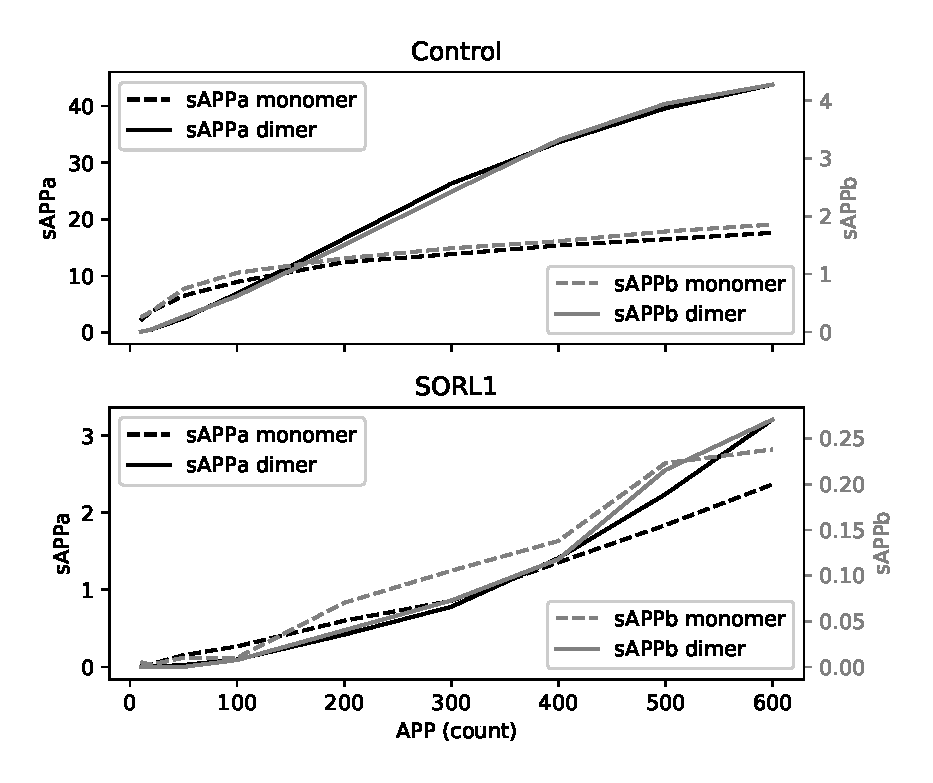
\includegraphics[width=8cm]{figure1.eps}
\caption{Plotted are average initial rates of the production of sAPPa, sAPPb, and their respective homodimers in the BEL2ABM simulation based on the amyloid beta cascade with varying initial number of APP agents. The sigmoidal curves observed in the control correspond to the cooperativity of the allosteric secretase dimers of sAPPa and sAPPb. Perturbation with SORL1 inhibits oligomerization, shown by the loss of sigmoidal shape, as well as causing significant decrease in the production of each of sAPPa, sAPPb, and their respective homodimers.
\textbf{Settings} alpha secretases: 10; alpha secretase dimers: 10; beta secretases: 1; 
beta secretase dimers: 1; SORL1: 3, 300 (only B); APP binding sites of allosteric enzymes: 2; binding 
strengths: 95\%; high lifespans so few molecule dies during experiment; 400 replicate runs at each APP 
concentration.}
\label{fig:01}
\end{figure}

\section{Discussion}
Because BEL2ABM produces inherently qualitative models, several constraints must be considered during their evaluation. The magnitude of the results can not be directly compared to experimental results or mathematical models such as the ODE system provided by Schmidt {\it et al.} because time and space are only artificially incorporated during simulation. Thus, we only expect to observe similar behavioral patterns of a real biological system.

NetLogo and other common simulation environments allow users to modify various simulation parameters in order to improve the adherence of an ABM to experimental data. While this allows users to the benefit of exploring based on their intuition, systematic optimization becomes a combinatorial problem for larger and more complex systems. BEL2ABM includes some semi-automatic parameter optimization methods and can be theoretically run with an optimization procedure like a grid search, but future work will include developing and encoding more biologically-driven optimization procedures in an ontology, like HuPSON, that can be leveraged to more automatically build relevant models. Further, the burden of choosing the most relevant and informative knowledge assemblies for BEL2ABM may be eased by the hypothesis generation procedures in upcoming BEL frameworks like PyBEL \citep{Hoyt17}.

With these restrictions in mind, we have shown that it is possible to dynamize a 
static knowledge assembly model, enable a user to qualitatively reproduce the behavior a biological system, and modify model parameters in order to make further investigations. 

\section*{Funding}

This work has been supported by the B-IT Foundation.

Conflict of Interest: none declared.

\begin{thebibliography}{}

\bibitem[Alden {\it et~al}., 2014]{Alden14}
Alden, K. J., et al. (2014). Applying spartan to Understand Parameter Uncertainty in Simulations. R Journal, 6(2), 63-80.

\bibitem[Catlett {\it et~al}., 2013]{Catlett13}
Catlett, N. L., et al. (2013). Reverse causal reasoning: applying qualitative causal knowledge to the interpretation of high-throughput data. BMC Bioinformatics, 14(1), 340.

\bibitem[G{\"u}ndel {\it et~al}., 2013]{Gundel13}
G{\"u}ndel, M., et al. (2013). HuPSON: the human physiology simulation ontology. Journal of Biomedical Semantics, 4, 35. 

\bibitem[Hoyt {\it et~al}., 2017]{Hoyt17}
Hoyt, et al. (2017), PyBEL: a computational framework for Biological Expression Language, Bioinformatics, btx660.

\bibitem[Hucka {\it et~al}., 2003]{Hucka03}
Hucka, M., et al. (2003). The systems biology markup language (SBML): a medium for representation and exchange of biochemical network models. Bioinformatics (Oxford, England), 19(4), 524-531.

\bibitem[Schmidt {\it et~al}., 2012]{Schmidt12}
Schmidt, V., et al. (2011). Quantitative modelling of amyloidogenic processing and its influence by SORLA in Alzheimer's disease. The EMBO Journal, 31(1), 187-200.

\end{thebibliography}
\end{document}
